\documentclass[12pt]{report}
\usepackage[utf8]{inputenc}
\usepackage{tabularx} % extra features for tabular environment
\usepackage{amsmath,amssymb,amsthm}  % improve math presentation
\usepackage[ruled,vlined]{algorithm2e}
\usepackage{caption}
\usepackage{subcaption}
\usepackage[hyphens]{url}
\newcommand{\E}{\mathrm{E}}
\newcommand{\Var}{\mathrm{Var}}
\newcommand{\Cov}{\mathrm{Cov}}
\newcommand{\Cor}{\mathrm{Cor}}
\DeclareMathOperator*{\argmin}{argmin}
\DeclareMathOperator*{\argmax}{argmax}
\newcommand\norm[1]{\left\lVert#1\right\rVert}
\newcommand\myleqa{\mathrel{\overset{\makebox[0pt]{\mbox{\normalfont\tiny\sffamily (a)}}}{\leq}}}
\newcommand\myleqb{\mathrel{\overset{\makebox[0pt]{\mbox{\normalfont\tiny\sffamily (b)}}}{\leq}}}
\newcommand\myleqc{\mathrel{\overset{\makebox[0pt]{\mbox{\normalfont\tiny\sffamily (c)}}}{\leq}}}
\newcommand\myeqa{\mathrel{\overset{\makebox[0pt]{\mbox{\normalfont\tiny\sffamily (a)}}}{=}}}
\newcommand\myeqb{\mathrel{\overset{\makebox[0pt]{\mbox{\normalfont\tiny\sffamily (b)}}}{=}}}
\usepackage{graphicx} % takes care of graphic including machinery
\usepackage{cite}
\usepackage[margin=1in,letterpaper]{geometry} % decreases margins
\usepackage[final]{hyperref} % adds hyper links inside the generated pdf file
\hypersetup{
	colorlinks=true,       % false: boxed links; true: colored links
	linkcolor=black,        % color of internal links
	citecolor=black,        % color of links to bibliography
	filecolor=magenta,     % color of file links
	urlcolor=black         
}
\usepackage{setspace}
\doublespacing

\begin{document}

\title{
{
\includegraphics[width=0.7\columnwidth]{university.jpg}}\\
{Greedy Principal Flows}\\
{\large National University of Singapore}\\
}
\author{Sebastian Lie}
\date{05 March 2021}
\maketitle

\chapter*{Acknowledgements}
My 7 soft toys. And my desk lamp for being the light of my life.

\chapter*{Abstract}

Principal Flows are a great tool to use when we want to extend the 
notion of Principal Component Analysis to multivariate high dimensional data that 
lie on non-linear lower dimensional manifolds.
This is especially since principal flows are curves on a manifold 
that move along a path of maximal variation of the data, and capture forms of
variation that would escape Principal Component Analysis.
Principal flows were originally obtained by solving a problem
in variational calculus using the Euler-Lagrange method. 
In this thesis, we explore the use of a novel, simpler approach to constructing 
principal flows: a greedy approach.
Furthermore, since after rotation, centering, translation 
and normalisation, vectors can be viewed as points on the hypersphere, 
we restrict this problem to constructing principal flows on hypersphere.
Let us call this new approach the greedy principal flow.
We test the effectiveness of our new principal flow on toy data, and
explore the patterns of variation it finds in real world data. Our results show that
our greedy principal flow retains the same effectiveness as the original, and
finds new, meaningful patterns in existing real world data.


\iffalse
The problem of dimension reduction arises in many areas: 
machine learning, data compression, scientific visualization, pattern recognition
and more. Some of the data in these areas 

While popular linear dimension reduction algorithms like Principal Component Analysis
have been successful, they often miss out essential information 
for some data higher dimensional data but can be viewed as lying on a lower dimensional 
manifold
\fi

\newpage
\tableofcontents
\listoffigures
\newpage

\chapter{Introduction}

\section{Motivation}

With the advent of Big Data, and the rise in popularity of data science,
machine learning has been used successfully to solve a variety of problems, 
such as regression and classification problems. However, machine learning
can also be used in a more subtle, but no less important way: to discover patterns
in the data and glean more information from it. Among methods that have this aim, 
Principal Component Analysis is the most popular, taught in almost every
machine learning course. It does however, have a glaring weakness: it does 
not perform well when the data we are working with is sampled from a non-linear manifold.
\\
This, however is remedied with the principal flow algorithm: 
it constructs a curve that at each local point moves in the direction of
maximal variation and retains canonical PCA interpretation in euclidean space.
Yet, this method is not easy to obtain, having to solve a problem in variational calculus. 
What if we could construct this curve with a greedy approach? 
Could the curve constructed still function as a principal flow? 
How would it perform on real world data and what new patterns of variation could it 
yield? These are some of the questions that motivated this thesis.\\
The first chapter outlines notations and some technical definitions. The 
second is a literature review of popular methods in dimension reduction. 
The third is where we explain how the greedy principal flow is constructed and 
the fourth chapter is where we present and analyse
our results after applying the greedy principal flow on toy and real world data.

\newpage

\section{Notation}

\begin{table}[ht]
\begin{tabular}{|l|l|}
\hline
\textbf{Notation} & \textbf{Explanation}                                      \\ \hline
$\mathbb{R}^D$    & $D$ dimensional euclidean space.                      \\ \hline
$\mathbf{X}$        & Data matrix of dimensions $n \times D$               \\ \hline
$\mathbf{X}_c$        & Centered Data matrix of dimensions $n \times D$                \\ \hline
$D$                & Dimension of the high-dimensional data.                \\ \hline
$d$               & Dimension of the manifold embedded in $D$ dimensional space \\ \hline
$\mathcal{M}^d$    & A connected and complete $d$-dimensional manifold
                   embedded in $\mathbb{R}^D$                                 \\ \hline
$p$               & A point on the manifold, $\mathcal{M}^d$.            \\ \hline
$\mathbf{v}$        & A vector.                                         \\ \hline
$T_p\mathcal{M}$    & The Tangent space of a point $p$ on $\mathcal{M}^d$.   \\ \hline
$\mathbf{C}$        & A Covariance matrix.                               \\ \hline
$\mathbf{C}_h(p)$   & A local tangent covariance matrix with scale $h$ 
\\ & of data on $T_p\mathcal{M}$.    \\ \hline
$\{x_1,...x_n\}$  & A collection of $n$ data points in $D$ dimensions. 
They are also the rows of $\mathbf{X}$  \\ \hline
$\mathbf{1}$      & A vector of $1$s.                                   \\ \hline
$\mathbf{I}$      & The identity matrix.                               \\ \hline
$\mathbf{X}^T$    & Transpose of $\mathbf{X}$.                          \\ \hline
$\mathbf{X}_{(d)}$ & $d$ dimensional representation of $\mathbf{X}$      \\ \hline
$\mathbf{V}$    & The matrix of eigenvectors of $\mathbf{C}$, 
where eigenvectors are columns and \\ & are sorted in descending order of their eigenvalues.  \\ \hline
$\mathbf{\Lambda}$    & The diagonal matrix of eigenvalues of $\mathbf{C}$, 
sorted in descending order.        \\ \hline
$\mathbf{V}_{(d)}$ & $d$ dimensional representation of $\mathbf{X}$      \\ \hline
$\mathbf{S}$    & Squared dissimilarity matrix of the data in $\mathbf{X}$ 
of dimension $n \times n$, \\ & calculated with euclidean distance. \\ \hline
$\otimes$    & Outer Product \\ \hline
\end{tabular}
\end{table}

\newpage

\section{Definitions}

\subsection{Vector Fields}
A vector at point $\mathbf{x}$, $\mathbf{x} \in \mathbb{R}^{D}$ is a pair 
$\mathbf{a} = (\mathbf{x}, \mathbf{v}), \ \mathbf{v} \in \mathbb{R}^{D}$, 
such that $\mathbf{v}$ is the vector $\mathbf{v}$ translated 
so that its tail is at $\mathbf{x}$ instead of the origin. 
All vector operations are defined such that the first item of 
the pair remains the same, 
and the second item is the result of the operation. 
The length and angle between two vectors are the same 
as normal vectors rooted in the origin.\\
\textbf{Definition:} A \textit{vector field} $\mathbf{F}$ on 
$U \subset \mathbb{R}^{D}$ is a function which assigns to each point
of $U$ a vector at that point. Then
$$\mathbf{F}(\mathbf{x}) = (\mathbf{x}, F(\mathbf{x}))$$ for some function 
$F: U \longrightarrow \mathbb{R}^{D}$. Vector fields on 
$\mathbb{R}^{D}$ are often most easily described by 
specifying this associated function $F$.
A pictoral example of a vector field is below.
\begin{figure}[ht]
    \begin{center}
        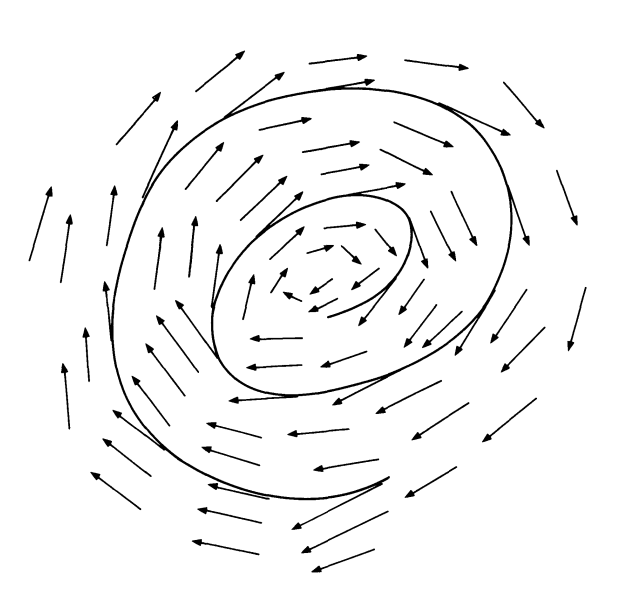
\includegraphics[scale=0.5]{fig2.5.PNG}
        \caption{An example of a vector field, $\mathbb{R}^3$}
        \label{fig:vectorfield}
    \end{center}
\end{figure}

\newpage

\subsection{Logarithm Maps}
\textbf{Logarithm Map:} For each $p \in \mathcal{M}^d$, let
$$log_p(x):\mathcal{M}^d\longrightarrow T_p\mathcal{M}$$
be the logarithm map. The log map is a function that projects a point $x$ 
on the manifold $\mathcal{M}^d$ onto $T_p\mathcal{M}$,
by producing a vector on $T_p\mathcal{M}$ which indicates the direction in which $p$
should move to obtain the projection of $x \in \mathcal{M}^d$ onto $T_p\mathcal{M}$.\\
\\
\textbf{Exponential Map:} For each $p \in \mathcal{M}^d$, let
$$exp_p(\mathbf{v}): T_p\mathcal{M} \longrightarrow \mathcal{M}^d$$
be the exponential map. Exponential maps are the inverse of the logarithm maps.
Let the vector $\mathbf{v}$ be the vector from $p$ to the point $t$ on $T_p\mathcal{M}$ we
wish to project onto $\mathcal{M}^d$. Then the exponential map moves along
the geodesic on $\mathcal{M}^d$ that mirrors the direction of $\mathbf{v}$
on $T_p\mathcal{M}$ and finds the projection of $t$ on $\mathcal{M}^d$.

\subsection{Tangent Space}
To define the tangent space we refer to the diagrams below.\\
\begin{figure}[ht]
\centering
\begin{subfigure}{.5\textwidth}
    \centering
    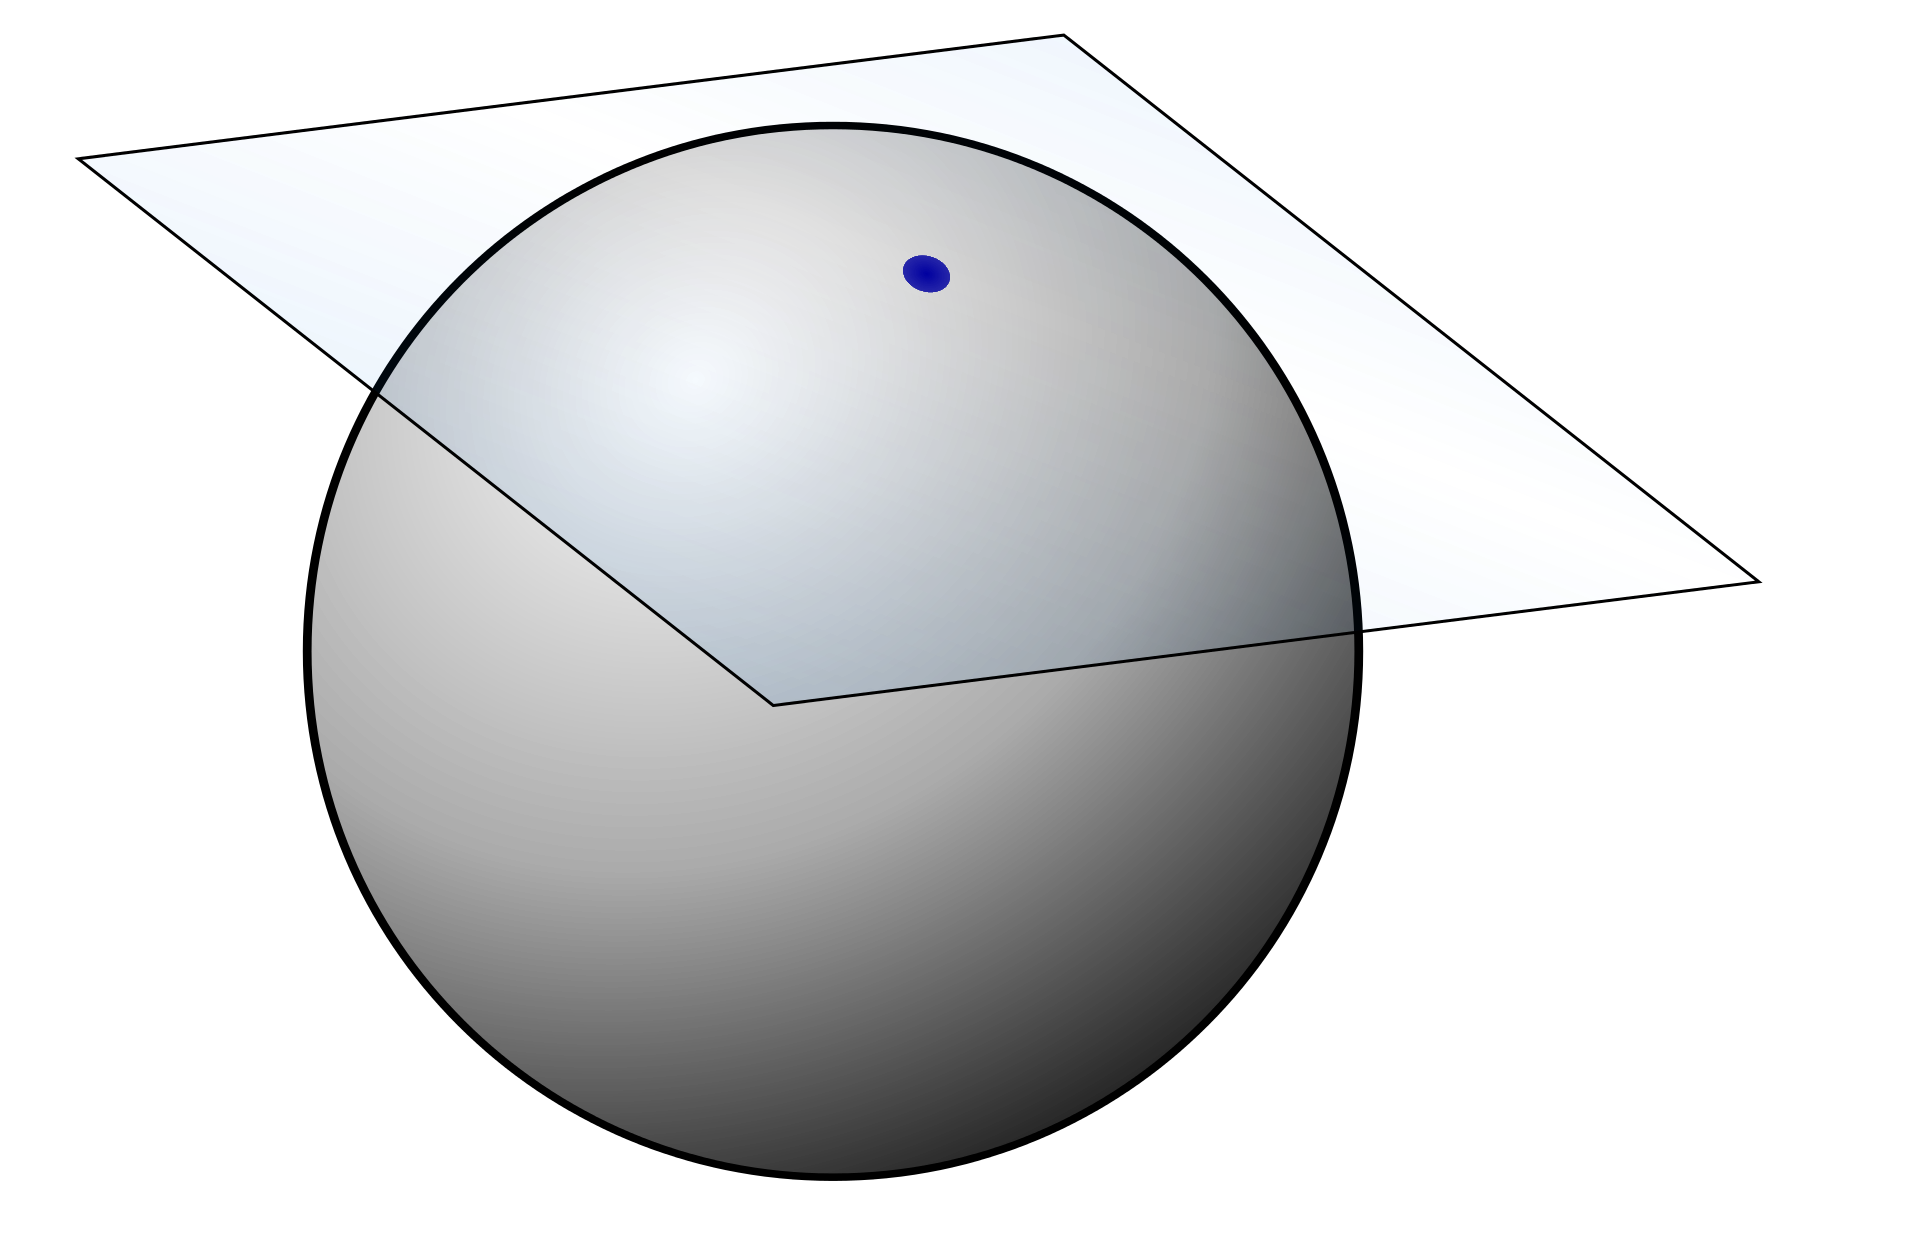
\includegraphics[scale=0.1]{tangent_space.png}
    \caption{Tangent Space of a Sphere\\ Obtained from \cite{tanspaceimg2}}
    \label{tanspacesphere}
\end{subfigure}%
\begin{subfigure}{.5\textwidth}
    \centering
    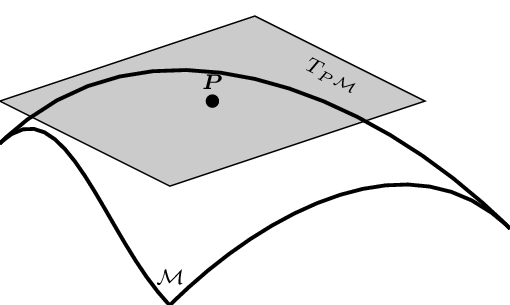
\includegraphics[scale=0.35]{tangent_space2.png}
    \caption{Close-up of the Tangent space in (a),\\ \ Obtained from \cite{tanspaceimg}}
    \label{tanspacemanifold}
\end{subfigure}
\caption{Illustration of a Tangent Space}
\label{fig:tanspaces}
\end{figure}
Let the sphere be the manifold, $\mathcal{M}^d$, and let $T_p\mathcal{M}$ 
be the plane tangent to $\mathcal{M}^d$. Let the blue point be $p$.
This is to say that the tangent space of some manifold $\mathcal{M}^d$
$log_p$ would then project points from $\mathcal{M}^d$ to the hyperplane,
and $exp_p$ would project points from $T_p\mathcal{M}$, the hyperplane, to $\mathcal{M}^d$.
Any vectors lying in this hyperplane are in the tangent space,
of $\mathcal{M}^d$ at $p$.


\subsection{Geodesics}

Geodesics are curves on $\mathcal{M}^d$
which play the same role as straight
lines in $\mathbb{R}^d$. They can be thought of as the "shortest path"
between two points on the manifold, $\mathcal{M}^d$.\\
\iffalse
or\\
\\
A geodesic on a $d$-dimensional manifold $\mathcal{M}^d \subset \mathbb{R}^D$ is a
parametrized curve $\alpha: I\longrightarrow M$ whose acceleration is everywhere
orthogonal to $\mathcal{M}^d$. Thus a geodesic is a curve in S which always goes" straight ahead" in
the surface,  Its acceleration serves only to keep it in the surface. It has no
component of acceleration tangent to the surface.\\
\fi
The Euclidean distance between two points $p, q$ 
is defined as $\norm{p-q}$, or the 2-norm of the vector $p - q$.
Geodesic distance extends this concept of Euclidean, straight line distance
in the Euclidean space to Manifolds. 


\subsection{Eigenvalues and Eigenvectors}
\textbf{Definition}: Let $\mathbf{C} \in \mathbb{R}^{D \times D}$. 
Then a non-zero vector $\mathbf{v}$ is an eigenvector of $\mathbf{C}$ 
if there exists some scalar $\lambda$ such that $\mathbf{C}\mathbf{v} = \lambda \mathbf{v}$. 
Then $\lambda$ is known as the eigenvalue corresponding to vector $\mathbf{v}$.\\
Here we also note that for any two eigenvectors $v_i$ and $v_j$, $i \neq j$, $v_i \cdot v_j = 0$, 
or any two eigenvectors are orthogonal to each other, and that $v_i \cdot v_i = 1$.

\subsection{Diagonalisation}
We say that a matrix, $\mathbf{C}$, is diagonalisable if there exists 
an orthonormal matrix such that the rows of that orthonormal matrix 
are the eigenvectors of $\mathbf{C}$, and a diagonal matrix 
$\mathbf{\Lambda}$ whose diagonal entries are the eigenvalues of $\mathbf{C}$.
In the context of this report, we only consider 
the eigendiagonalisation of some covariance matrix 
$\mathbf{C} \in \mathbb{R}^{D \times D}$,
which is symmetric and thus, always diagonalisable. Formally,
the eigendiagonalisation of $\mathbf{C}$ is given by:
$$\mathbf{C} = \mathbf{V}\mathbf{\Lambda}\mathbf{V}^T$$

\chapter{Literature Review}

\section{Linear Dimension Reduction}

\subsection{Principal Component Analysis}

\iffalse
Note that centering each variable is the same as finding the "mean" 
observation $\bar{x} = \frac{1}{n}\sum^n_{i=1}x_i$, 
and subtracting that from every observation: $x_i - \bar{x}$, 
since $\bar{x}_i$ is the mean of the i-th variable.
This is done by calculating the covariance matrix 
of the centered data, $\mathbf{C}$, then 
computing the eigendiagonalisation of $\mathbf{C}$ 
and compute the dot product of the original 
data matrix by the $d$ eigenvectors associated with the 
$d$ largest eigenvalues.
\fi
\textbf{Principal Component Analysis(PCA)} tries to obtain a 
lower-dimensional representation of the data 
that retains as much variation as possible present in the data set. 
PCA relies on constructing principal components (PCs): 
new variables that are linear combinations of the original variables 
that have first been centered.
These PCs are uncorrelated (orthogonal) and ordered in descending order 
by the amount of variability of the original data retained.
Thus, PCA reduces some high-dimensional data of dimension $D$ 
to $d$ by computing the first $d$ PCs.\\
We compute these PCs by first centering the data matrix, $\mathbf{X}$, and
obtaining $\mathbf{X}_c$. Next we compute the covariance matrix of 
the centered data matrix: $\mathbf{C}$.
Then we compute the eigendiagonalisation of $\mathbf{C}$,
and obtain $\mathbf{V}_d$, the $d$ eigenvectors associated 
with the $d$ largest eigenvalues. Here, we note that these $d$ eigenvectors
are the $d$ principal directions: directions onto which data is projected to
obtain the $d$ PCs.
Finally, we construct the $d$ PCs by computing $\mathbf{X}\mathbf{V}_d$.
\\
The PCA algorithm is outlined below. We assume for simplicity that the 
following functions are available:
$center$ that centers a given matrix, $covariance$ that computes the covariance
of a given matrix, and $diagonalise$ which compute the $d$ 
eigenvectors associated with the $d$ largest eigenvalues.
\begin{algorithm}
\KwResult{$\mathbf{X}_{(d)}$, the $d$ dimensional representation of $\mathbf{X}$, which are the d PCs}
    $\mathbf{X}_c = center(\mathbf{X})$\;
    $\mathbf{C} = covariance(\mathbf{X}_c)$\;
    $\mathbf{V}_d = diagonalise(\mathbf{C}, d)$\;
    $\mathbf{X}_{(d)} = \mathbf{X}\mathbf{V}_{d}$\;
    \Return{$\mathbf{X}_{(d)}$}
    \caption{PCA($\mathbf{X}$, $d$)}
\end{algorithm}

\subsection{Classical MDS, Euclidean Distance}
\textbf{Multidimensional Scaling (MDS)}'s 
main aim is find some $d$ dimensional representation of the
original data, $\mathbf{X}_{(d)}$,
that minimises the discrepancy between the pairwise distances 
of $\mathbf{X}$ and $\mathbf{X}_{(d)}$, 
given the squared matrix of pairwise distances of $\mathbf{X}$, $\mathbf{S}$.\\
Since dissimilarities do not change under translations, 
we can assume that $\mathbf{X}$ has column means equal to 0. 
Let $\mathbf{B} = \mathbf{X}\mathbf{X}^T$ be the gram matrix.
Let $\mathbf{J}$ be the centering matrix: 
$\mathbf{J} = \mathbf{I} - n^{-1}\mathbf{1}\mathbf{1}^T$, where 
$\mathbf{I} \in \mathbb{R}^{n \times n}$ and $\mathbf{1} \in \mathbb{R}^{n \times 1}$
Then, we run MDS by first computing  
$\mathbf{B} = -\frac{1}{2}\mathbf{J}\mathbf{S}\mathbf{J}$.
Then computing the eigendecomposition of $\mathbf{B}$.
$\mathbf{B} = \mathbf{V}\mathbf{\Lambda}\mathbf{V}^T$. 
From the original $\mathbf{V}$ we take the first $d$ columns: $\mathbf{V}_d$
and the first $d \times d$ submatrix of $\mathbf{\Lambda}$: $\mathbf{\Lambda}^{1/2}_d$.
Finally, we compute
$\mathbf{X}_{(d)} = \mathbf{V}_d\mathbf{\Lambda}^{1/2}_d$ to 
obtain the $d$-dimensional representation of the original data, $\mathbf{X}$. 
The MDS algorithm is outlined below. Assume we have a function $diagonalise$ which
computes returns the first $d$ columns of $\mathbf{V}$ and 
the $d \times d$ submatrix of $\mathbf{\Lambda}$.\\
\begin{algorithm}
\KwResult{$\mathbf{X}_{(d)}$, the $d$ dimensional representation of $\mathbf{X}$}
    $\mathbf{J} = \mathbf{I} - n^{-1}\mathbf{1}\mathbf{1}^T$\;
    $\mathbf{B} = -\frac{1}{2}\mathbf{J}\mathbf{S}\mathbf{J}$\;
    $\mathbf{V}_d, \mathbf{\Lambda}_d = diagonalise(\mathbf{B}, d)$\;
    $\mathbf{X}_{(d)} = \mathbf{V}_d\mathbf{\Lambda}^{1/2}_d$\;
    \Return{$\mathbf{X}_{(d)}$}
    \caption{MDS($\mathbf{S}$, $d$)}
\end{algorithm}
Note that using Euclidean distances, the result of MDS is the same as PCA.
\newpage
\section{Non-Linear Dimension Reduction}

Non-linear dimensionality reduction methods are particularly useful 
when the multivariate data we obtain is sampled 
from a smooth non-linear manifold $\mathcal{M}^d$, 
e.g a manifold in an S-shape or a hypersphere. 
This class of methods obtain better estimates than linear methods like PCA and MDS,
especially for the data mentioned above. 
They are especially successful as certain data sets contain 
essential nonlinear structures that are invisible to PCA and MDS.

\newpage

\subsection{Isomap}

\textbf{Isomap}, introduced by Tenenbaum et al. \cite{isomap} is an extension 
of MDS to manifolds in which embeddings 
are optimized to preserve geodesic distances between pairs of data points.
It combines the major algorithmic features of PCA and MDS
— computational efficiency, global optimality, 
and asymptotic convergence guarantees — 
with the flexibility to learn a broad class of nonlinear manifolds.
Isomap achieves this by estimating the geodesic distance between data points, 
given only input-space distances, e.g euclidean distance between points.\\
This relies on the fact that for neighboring points, 
input-space distance provides a good approximation to geodesic distance. 
For faraway points, Isomap approximates geodesic distance 
by adding up a sequence of “short hops” between neighboring points, 
computed efficiently by finding shortest paths in a graph with edges 
connecting neighboring data points.\\
\iffalse
This approximation relies on the proof that for a 
sufficiently high density of data points, 
we can always choose a neighborhood size large enough 
that the graph will (with high probability) have a path not much longer 
than the true geodesic, but small enough to prevent edges 
that “short circuit” the true geometry of the manifold \cite{isomap}.\\
\fi
Like MDS, Isomap takes as input $\mathbf{S}$ but differs by first 
constructing the neighbourhood graph, $G$. We start by creating nodes for every 
data point $i$. Given some user input $K$,
for every point $i$, Isomap adds an edge between
the $i$ and another point $j$ with weight $S_{i,j}$ if $j$ is 
one of $i$'s $K$ nearest neighbours. We then run an all pairs shortest path 
algorithm on $G$ (we use FloydWarshall here), and obtain a new matrix 
$\mathbf{A}$, where $\mathbf{A}_{i,j}$ is the shortest distance from $i$ to $j$. 
This approximates geodesic distance between $i$ and $j$. 
Then we run $MDS(\mathbf{A}, d)$ from to obtain $\mathbf{X}_{(d)}$. \\
The algorithm is outlined below. For simplicity, 
assume we have a function $ConstructGraph$ which 
constructs the graph $G$ as explained above.
\begin{algorithm}
\KwResult{$\mathbf{X}_{(d)}$, the $d$ dimensional representation of $\mathbf{X}$}
    $G = ConstructGraph(\mathbf{S}, K)$\;
    $\mathbf{A} = FloydWarshall(G)$\;
    \Return{MDS($\mathbf{A}$, $d$)}
    \caption{Isomap($\mathbf{S}$, $d$, $K$)}
\end{algorithm}

\newpage

\subsection{Locally Linear Embeddding}

\textbf{Locally Linear Embedding (LLE)} introduced by 
Saul and Roweis \cite{lle} aims to construct 
a mapping from the $D$ dimensional 
original points to the $d$ dimensional reconstructed points
that preserves the local configurations of each point's nearest neighbors. 
Locally, LLE assumes the embedding is linear, 
and for each data point $p \in \mathbb{R}^D$, 
LLE uses a linear combination of its $K$ nearest neighbours 
to reconstruct a lower-dimensional $p_d \in \mathbb{R}^d$. \\
Let the set of the $i$-th point's $k$ nearest neighbours be $N^i_k$.
LLE starts by learning some weights from the $D$-dimensional data: 
$\mathbf{W}$ by minimizing the \textbf{Reconstruction Error} 
below using constrained linear fits.
$$\varepsilon (\mathbf{W}) = \sum_i^n|\mathbf{X}_i - \sum_{j \in N^i_k}^K \mathbf{W}_{ij} \mathbf{X}_j|^2$$
Here, $\mathbf{W}$ are the weights that best reconstruct each 
data point from it's $K$ neighbours, and
$\mathbf{W}_{ij}$ represents the contribution 
of the j-th data point in reconstructing the i-th one.
These weights obey an important symmetry: for any particular data point,
they are invariant to rotations, rescalings, and translations
of that data point and its neighbors.
They thus reflect intrinsic geometric properties 
of the data that are invariant to such transformations,
and therefore, we expect their characterization of local geometry in the 
original data space to be equally valid for local patches on the manifold.
This is what motivates our use of $\mathbf{W}_{ij}$ in reconstructing
the embedded manifold coordinates in $d$ dimensions. \\
Next, compute the vectors $\mathbf{Y}_i$ best 
reconstructed by the weights $\mathbf{W}_{ij}$ 
by choosing the $d$ dimensional coordinates of each output
that minimise the \textbf{Embedding Cost Function}: 
$$\Phi(\mathbf{Y}) = \sum_i |\mathbf{Y}_i - \sum_j \mathbf{W}_{ij}\mathbf{Y}_j|^2$$
At the end of LLE, each $D$-dimensional observation $\mathbf{X}_i$ 
is mapped to a $d$ dimensional $\mathbf{Y}_i$ 
representing global internal coordinates on the manifold.\\
\begin{algorithm}
\KwResult{$\mathbf{X}_{(d)}$, the $d$ dimensional representation of $\mathbf{X}$}
    First compute $N^i_k$ for all $x_i$\;
    $\mathbf{W} = argmin_{\mathbf{W}}\sum_i^n|x_i - \sum_{j \in N^i_k}^k \mathbf{W}_{ij} x_j|^2$\;
    $\mathbf{X}_{(d)} = argmin_{\mathbf{Y}}\sum_i |\mathbf{Y}_i - \sum_{j \in N^i_k}^k \mathbf{W}_{ij}\mathbf{Y}_j|^2$\;
    \Return{$\mathbf{X}_{(d)}$}
    \caption{LLE($\mathbf{X}$, $d$, $k$)}
\end{algorithm}

\subsection{Principal Geodesic Analysis}
\iffalse
by finding a sequence of lower-dimensional subspaces, 
which on manifolds are nested geodesic submanifolds 
that maximize the projected variance of the data. 
These submanifolds are called the principal geodesic submanifolds, 
which are analogous to linear subspaces in PCA.\\
Let $U \subset T_p\mathcal{M}$ be a neighbourhood of 0 in which our data, 
$\mathbf{X}$ lies, such that projection is well defined 
for all geodesic submanifolds of $exp_p(U)$.These principal geodesic submanifolds 
are obtained by first constructing an orthonormal basis of tangent vectors 
$v_1,...,v_d \in T_p\mathcal{M}$ that span the tangent space. 
These vectors are then used to form the principal geodesic subspaces 
$H_k$ where $H_k = exp_p(V_k)$, and $V_k$ is intersection of the 
subspace spanned by vectors $1..k$ and $U$.
subspace $V_k = span(\{v_1,...,v_k\})\bigcap U$.
\fi
Principal Geodesic Analysis(PGA) introduced here \cite{pga}, 
is a generalization of PCA to manifolds. 
The main aim of PGA is to describe some $D$ dimensional data that
lie on $\mathcal{M}^d$ embedded in $\mathbb{R}^D$.
Let $T_p\mathcal{M}$ be the tangent space of $\mathcal{M}^d$ 
at the intrinsic mean $p$ of the data. 
The intrinsic mean here is the extension of the concept 
of the mean in euclidean space to manifolds.
PGA aims to construct some principal geodesics that are analogous
to principal directions in PCA: the directions along which data is
projected to obtain a PC.\\
Instead of finding the principal geodesic however, Fletcher et al. prove that
we can approximate the $d$ geodesics along which maximal variation lies 
by projecting data from $\mathcal{M}^d$ to $T_p\mathcal{M}$ where 
$p$ is the intrinsic mean of $\{x_1,..x_n\}$
and then finding the 
$d$ eigenvectors associated with the $d$ largest eigenvalues of the 
covariance matrix of the projected data.\\
PGA begins with computing $p$ by first setting 
$p$ to a random data point, 
then iteratively obtaining a better estimate of $p$. Let $p_i$ be the 
estimate of $p$ at the i-th iteration.
At the i-th iteration, we compute the average of the vectors obtained 
using the $log_{p_{i-1}}(x_i), \forall x_i$ then setting $p_{i}$ 
as the projection of that average using $exp_{p_{i-1}}$.\\
After obtaining $p$, we calculate the vectors $u_i = log_p(x_i), \ \forall x_i$.
Next we calculate the covariance matrix 
$\mathbf{C} = \frac{1}{n} \sum^n_{i=1} u_iu_i^T$.
Finally we diagonalise $\mathbf{C}$ to obtain $\{v_k, \lambda_k\}$ 
the eigenvectors and eigenvalues respectively, 
which represent the principal directions 
in the tangent space $T_p\mathcal{M}$ and the variances.
The algorithm for PGA is outlined below.
\begin{algorithm}
\KwResult{$\{v_1,...v_D\} \in T_p\mathcal{M}$, principal directions and \\
Variances $\{\lambda_1,...\lambda_D\} \in \mathbb{R}$}
    $p = $ intrinsic mean of data $\{x_1,....x_n\}$\;
    $u_i = log_p(x_i)$\;
    $\mathbf{C} = \frac{1}{N}\sum^N_{i=1}u_i u_i^T$\;
    $\{v_1,...v_D\}, \{\lambda_1,...\lambda_D\} = $ eigenvectors and eigenvalues of $\mathbf{C}$\;
    \Return{$\{v_1,...v_D\}, \{\lambda_1,...\lambda_D\}$}
    \caption{PGA($\{x_1,...x_n\}$)}
\end{algorithm}

\chapter{Greedy Principal Flows}

\section{Goal Of Research}

The main objective for greedy principal flows is to quantify or describe 
multivariate data on the manifold: we cannot simply fit a line, 
as this is not Euclidean space.
Instead, we want some curve or path such that,
locally, it follows the path of maximal variation of the data in some neighbourhood, 
but globally also provides the path of maximal ``cumulative" variation of the data.
This problem has already been solved in \cite{principalflow}, 
where the principal flows were constructed by 
solving a problem in variational calculus. Here we note that we focus on 
the first order principal flow, which can be thought of as 
the manifold extension of the first PC in euclidean space.
Therefore, we focus instead on constructing the principal flow using a novel, 
simpler to implement approach: a greedy algorithm. 
Additionally, we simplify our approach further and 
assume that our data $\mathbf{X}$ is some $D$ dimensional
data lying on a hypersphere $\mathcal{M}^d$.
Thus, formally, our goal is to implement this simpler version of the
principal flow algorithm in a popular programming language, 
and experiment with the results that this implementation of the
principal flow algorithm. How would it describe various, popular multivariate
datasets? Could it find novel ways of describing popular,
existing high-dimensional data?

\section{Centroid Algorithm}
Before we get into our principal flow algorithm, we first need to 
establish our starting point. Since our principal flow 
follows the path of maximal variation of our data, 
we know it should pass through the centroid of the data. 
Thus, we first aim to estimate this centroid and use it as a starting point.
Although there are many ways of doing this,
including the method to find the intrinsic mean in chapter 2.2.3,
we opt to make use of the fact that 
the first PC passes through the centroid of the data. Thus, if we 
iteratively project all the data onto the tangent space of the hypersphere, 
find the 1st principal direction, move in that direction, 
and find the projected point on the hypersphere, we will eventually converge on the 
centroid. The algorithm to find the centroid is outlined below.
\begin{algorithm}
\KwResult{$p$, centroid of the data}
    $p = $ a random data point from $\{x_1,....x_n\}$\;
    \For{$i = 1 \to max\_iter$}{
        Compute $u_i = log_p(x_i)$ for all $x_i$,\;
        $\mathbf{C} = \frac{1}{N}\sum^N_{i=1}u_i u_i^T$\;
        $v_1 = $ eigenvector corresponding to the largest eigenvalue of $\mathbf{C}$\;
        $p' = p + \epsilon v_1$\;
        $p = exp_p(p')$\;
    }
    \Return{$p$}
    \caption{Centroid($\{x_1,...x_n\}$)}
\end{algorithm}

\iffalse
\textbf{Problem}:
With our starting point settled, we observe that the principal flow algorithm may run
into a problem: What if our data stretches all around the hypersphere? 
How do we deal with projecting
data through the sphere?\\
To solve this, instead of taking all data into consideration, 
we use a kernel function, $\mathcal{K}$ to choose a small neighborhood around
our current principal flow point, whose size is controlled by $h$. 
For our algorithm, we implement 2 choices of kernel functions: The binary kernel 
includes points in some neighbourhood and excludes points outside,
while the gaussian kernel weights points according to 
the gaussian distribution based on their distance from the original point.\\
Thus, we
project the data within some neighbourhood $\mathbf{X}$ onto the tangent space 
at the centroid, p: $T_p\mathcal{M}$. We use the logarithm map, $log_p$ to do this. 
Then the path of maximal variation in this neighbourhood of points 
is the first principal direction of this data from PCA. This direction 
is obtained by diagonalising the covariance matrix of the data on this tangent
space. \\
\textbf{Problem}:
This direction clearly is not accurate if we only move in this direction,
since it will eventually lead us out of the surface of the hypersphere, and even on the 
hypersphere, the neighbourhood of points may differ, and change the direction 
of the path of maximal variation.\\
Thus, instead of only using this direction, we move infinitesimally in this first direction,
then carry out the same procedure again. Thus we iteratively find the "local"
direction of maximal variation, move in that direction, and re-compute the next direction
of maximal variation. We continue doing this until we have obtained a flow through the
entire data set.\\
This does indeed follow the framework that isomap and LLE abide by
as well: that obtaining the best option locally becomes the best option globally as well. 
This is exactly the idea of this Greedy Principal flow algorithm. 
\fi
\section{Algorithm}

Now we move on to outlining and elaborating on the Principal flow algorithm.
Starting from the centroid of the data set, we first
project $\mathbf{X}$ onto the hyperplane
at $p$ (initially the centroid of the data lying on $\mathcal{M}^d$), $T_p\mathcal{M}$.
\iffalse
However, we realise we may run into a problem: 
What if our data stretches all around the hypersphere? 
How do we deal with projecting data through the sphere?\\
To solve this, instead of projecting all data, 
we use a kernel function, $\mathcal{K}$ to choose a small neighborhood around
our current principal flow point, whose size is controlled by scale parameter $h$. 
\fi
Here we may choose to project all our data, or use a kernel function, 
$\mathcal{K}$ to weight our data so that more emphasis is 
placed on points in some neighborhood around
$p$, whose size is controlled by scale parameter $h$, than outside it.
Intuitively, $h$ controls how sensitive the principal flow is to local data.
For our algorithm, we implement three choices of kernel functions: The binary kernel 
which weights points as one or zero depending on their distance from 
$p$, the gaussian kernel which weights points according to 
the gaussian distribution based on their distance from $p$ and
lastly the identity kernel, which sets all weights to be one.\\
Thus, we first apply our kernel function to the data, and obtain weights 
$\{w_i,....w_n\}$, then apply our log map $log_p$ to project our data on 
$\mathcal{M}^d$ obtaining a matrix of vectors on the tangent plane that point from $p$
to the projected points. These are our plane vectors $log_p(x_i)$.\\
Then we compute the covariance matrix of the plane vectors
using both our weights and our plane vectors
by the equation below obtained from \cite{principalflow}.
$$C_h(p) = \frac{1}{\Sigma_i \mathcal{K}_h(x_i,p)}\sum^n_{i=1}(log_p(x_i)\otimes log_p(x_i))\mathcal{K}_h(x_i,p)$$
We then perform eigendiagonalisation of the covariance matrix. 
Take the eigenvector $v_1$ corresponding to the largest eigenvalue $\lambda_1$. 
This indicates the direction of the principle flow. Let us call it
the principal direction. Here, $\lambda_1$ corresponds to the amount
of variance of our data in the direction of $v_1$.
This is where the ``greediness'' in 
our algorithm lies: since we choose at each step, the direction of maximum 
variance.\\
If this is the first iteration, we collect two points: 
one point when we move a step size of $\epsilon$ in the principal direction, 
and the other when we move a step size of $\epsilon$ in the 
opposite of the principal direction. We then project both points back onto 
$\mathcal{M}^d$, using $exp_p$. 
Set $p$ to be the first point, and $p\_opp$ to be the second. 
Otherwise, we check that this principal direction is in the same 
direction as the previous principal direction, and if not, apply a negative sign
to the principal direction. 
As above we now move a step size of $\epsilon$ in the principal direction, 
then project both points back onto 
$\mathcal{M}^d$, using $exp_p$.\\
We repeat the procedure above until the maximum iterations is reached.
Then we set $p = p\_opp$ and repeat the procedure above, with the 
exception that we only produce one point at every iteration. This is to say, 
we only repeat what is done in the second iteration onwards, and stop when the 
maximum number of iterations is reached. 
The Greedy Principal Flow algorithm is outlined below.

\begin{algorithm}
\KwResult{$p_i$, points on the principal flow}
    \For{$i = 1 \to max\_iter$}{
        
        \If{$i == 1$}{
            $\{w_i,....w_n\} = \mathcal{K}(h, p, \{w_i,....w_n\}$\;
            $\mathbf{C}_h(p) = \frac{1}{\Sigma_i w_i}\sum^n_{i=1}(log_p(x_i)\otimes log_p(x_i))w_i$\;
            $\{v_1,...,v_n\}, \{\lambda_1,...\lambda_n\} = diagonalise(\mathbf{C}_h(p))$\;
            $first\_direction = v_1$\;
            $p = exp_p(p + \epsilon v_1)$\;
            $p\_opp = exp_p(p - \epsilon v_1)$\;
            $v_1\_past = v_1$\;
        }
        \Else{
            $\{w_i,....w_n\} = \mathcal{K}(h, p, \{w_i,....w_n\}$\;
            $mathbf{C}_h(p) = \frac{1}{\Sigma_i w_i}\sum^n_{i=1}(log_p(x_i)\otimes log_p(x_i))w_i$\;
            $\{v_1,...,v_n\}, \{\lambda_1,...\lambda_n\} = diagonalise(\mathbf{C}_h(p))$\;
            \If{$cos^{-1}(v_1^Tv_1\_past > \pi/2$}{
                $v_1 = -v_1$\;
            }
            $p = exp_p(p + \epsilon v_1)$ update p\;
        }
    }
    $p = p\_opp$\;
    \For{$i = 1 \to max\_iter$}{
        $\{w_i,....w_n\} = \mathcal{K}(h, p, \{w_i,....w_n\}$\;
        $mathbf{C}_h(p) = \frac{1}{\Sigma_i w_i}\sum^n_{i=1}(log_p(x_i)\otimes log_p(x_i))w_i$\;
        $\{v_1,...,v_n\}, \{\lambda_1,...\lambda_n\} = diagonalise(\mathbf{C}_h(p))$\;
        \If{$cos^{-1}(v_1^Tv_1\_past > \pi/2$}{
            $v_1 = -v_1$\;
        }
        $p = exp_p(p + \epsilon v_1)$\;
    }
    \Return{$p$}
    \caption{GreedyPrincipalFlow($\{x_1,...x_n\}$, $\mathcal{K}$, $max\_iter$, $h, \epsilon$)}
\end{algorithm}

\newpage 
\section{Extension: Greedy Principal Boundary}
In the section above, we have already seen the principal flow.
Now we extend the idea of Principal flows to attempt to find some boundary of the data.
Let us assume that the data is contained on some ellipse of the manifold
$\mathcal{M}^d$. Then our aim is to find some boundary around this ellipse. We proceed 
similarly to the principal flow, except that 
we now save $v_1, v_2, \lambda_1, \lambda_2$
when we diagonalise $\mathbf{C}_{h}(p)$.
and use them to compute the boundaries of data.\\
Then at each iteration, the boundary $b$ is calculated before $p$ 
is updated by $b_1 = exp_p(p + \frac{\lambda_2}{\lambda_1}*radius*v_2)$ and
$b_2 = exp_p(p - \frac{\lambda_2}{\lambda_1}*radius*v_2)$
where radius is a user specified parameter. Intuitively, 
we try to move a distance in the direction of $v_2$ orthogonal to the principal flow
that approximates the radius of the ellipse that contains the data, $\mathbf{X}$.

\chapter{Applications}
Writing the algorithm is meaningless without testing that it also functions 
as we want it to. First we start with simple applications on toy data to confirm that 
our algorithm works as intended, then we apply it on some real world data to show
how the principal flow can be used there as well.

\section{Toy Data}

\subsection{Without Noise}

As a sanity check or proof of concept of our principal flow, 
we first want to test our algorithm on some toy data that we know 
lies on the three-dimensional unit sphere. This will help us visualise the flow created
and determine if it follows the pattern of the data, 
and thus act as a proof of concept of
our algorithm. We generate some data artificially.

\begin{figure}[ht]
    \centering
    \begin{subfigure}{.5\textwidth}
        \centering
        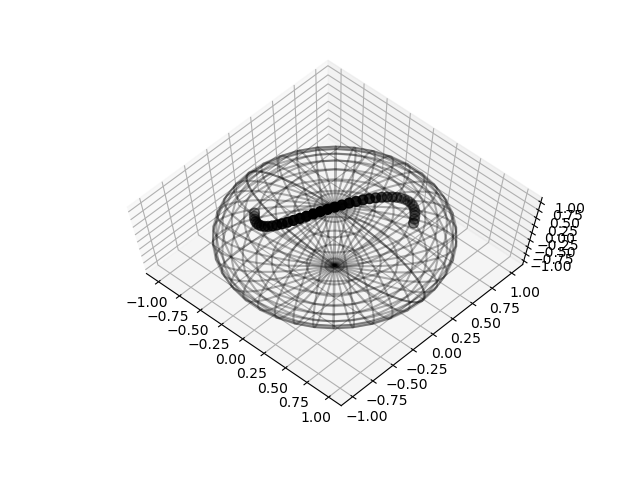
\includegraphics[scale=0.5]{Data_13.png}
        \caption{Toy data 13, $\mathbb{R}^3$}
        \label{fig:toydata}
    \end{subfigure}%
    \begin{subfigure}{.5\textwidth}
        \centering
        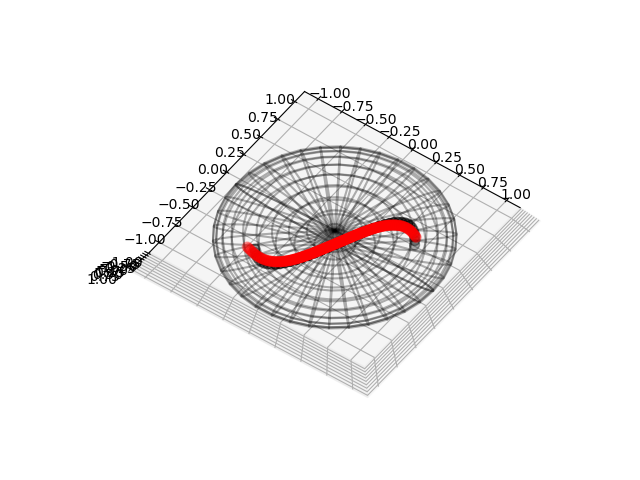
\includegraphics[scale=0.5]{single_flow_13.png}
        \caption{Principal Flow on Toy Data, $\mathbb{R}^3$}
        \label{fig:pflowtoy}
    \end{subfigure}
    \caption{Principal flow, no noise}
    \label{fig:nonnoiseflows}
    \end{figure}

\newpage

For example, this dataset is created by setting the first coordinate of the 
i-th point, $x_{i, 1} = \frac{i-n/2}{n}$, then $x_{i, 2} = sin(4*x_{i, 1})/2$, 
and the third to $x_{i, 3} = \sqrt{1-x_{i, 1}^2 - x_{i, 2}^2}$, 
where n is the number of points we want to generate.\\
Now that we have seen the Toy Data, let us apply the Principal Flow 
algorithm to the data above.
This 3D plot shows the original data in black, and the principal flow in 
\textcolor{red}{red}.
With some tuning of h, the size of the neighbourhood, we can see that we have constructed
a principal flow that follows the original data almost
exactly, reconstructing an S with some slight differences at the curves of the s-shape of
the original data.
We have now seen that proof that our principal flow algorithm works:
it is able to accurately reconstruct the toy data, 
the s curve on the sphere.

\subsection{With Noise}

Next, gaussian noise was added to the S-shaped data on the sphere to create a noisy dataset.
Then we fitted a principal flow to this noisy data.
\iffalse
NOte: run noisy flow again! With same seed this time....
\fi
\begin{figure}[ht]
\centering
\begin{subfigure}{.5\textwidth}
    \centering
    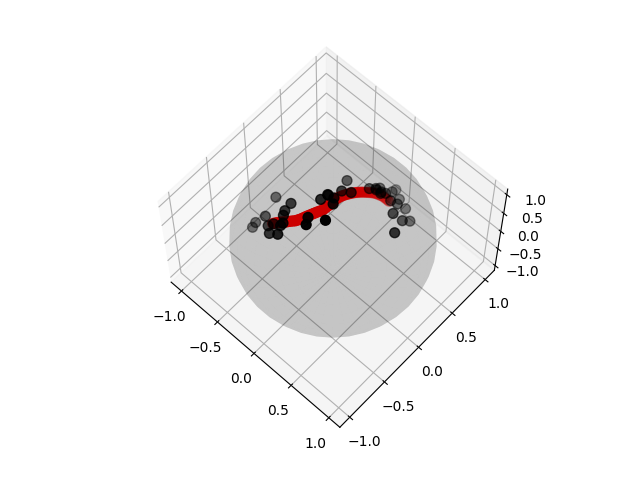
\includegraphics[scale=0.5]{noisy_13_binary.png}
    \caption{Flow on Noisy Data using binary kernel}
    \label{noisybinary}
\end{subfigure}%
\begin{subfigure}{.5\textwidth}
    \centering
    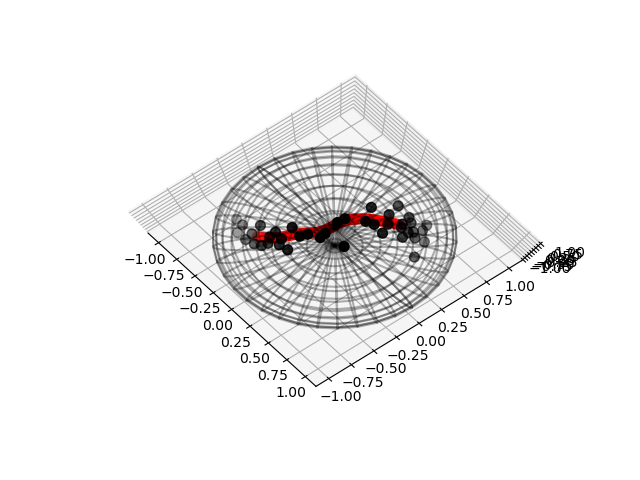
\includegraphics[scale=0.5]{noisy_13_gaussian.png}
    \caption{Flow on Noisy Data using gaussian kernel}
    \label{noisygaussian}
\end{subfigure}
\caption{Principal flow, noisy data}
\label{fig:noisyflows}
\end{figure}

We can see that the principal flow obtained seems to follow the new pattern 
of variation in the data: from the more dense cloud of points on the left, to the curve of
the points in the center to the other dense cloud of points on the right.
We can see from these examples that even with noise, our algorithm is able to discern 
the pattern of the data.

\subsection{Boundary Flow with Noise}

Next we test out our extension, our algorithm for our principal boundary.
Since we need a ``cloud" of data, we apply some gaussian noise on the data from above,
and then run our principal boundary algorithm on it. Let the principal flow
be the curve in red, and the boundaries be in blue and green.

\begin{figure}[ht]
    \begin{center}
        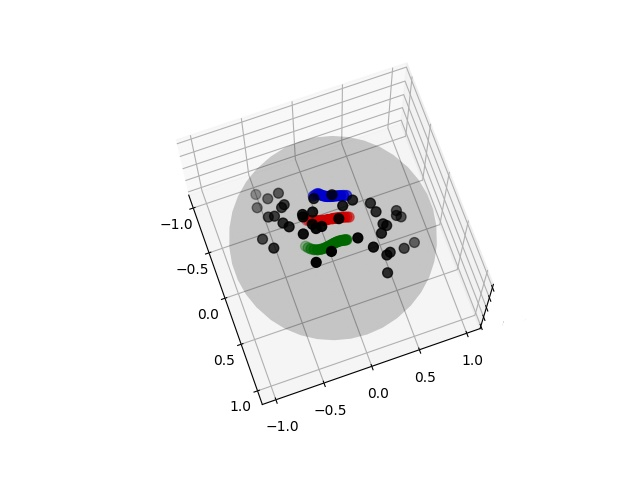
\includegraphics[scale=0.5]{noisy_boundary_flow13.jpg}
        \caption{Boundary Flow on noisy data}
        \label{fig:boundaryflows}
    \end{center}
\end{figure}

With some tuning, we obtain these three curves: we can see that the principal flow
is in the middle of the dataset, while the boundary flows accompany it in parallel
and even form to the shape of the cloud of data, bending outwards
when there is a point beyond it. Through this graph, we can see how the principal
boundary can work and be shaped by the shape of the cloud of data.

\section{Real World Data}

Our results on artificial data are promising, however, it means little
if there are no real-world applications for our greedy principal flow.

\subsection{MNIST}
 
We first test the principal flow algorithm on the MNIST dataset, a rite of passage
for machine learning algorithms. The MNIST dataset is a set of handwritten digits.\\  
\begin{figure}[ht]
    \begin{center}
        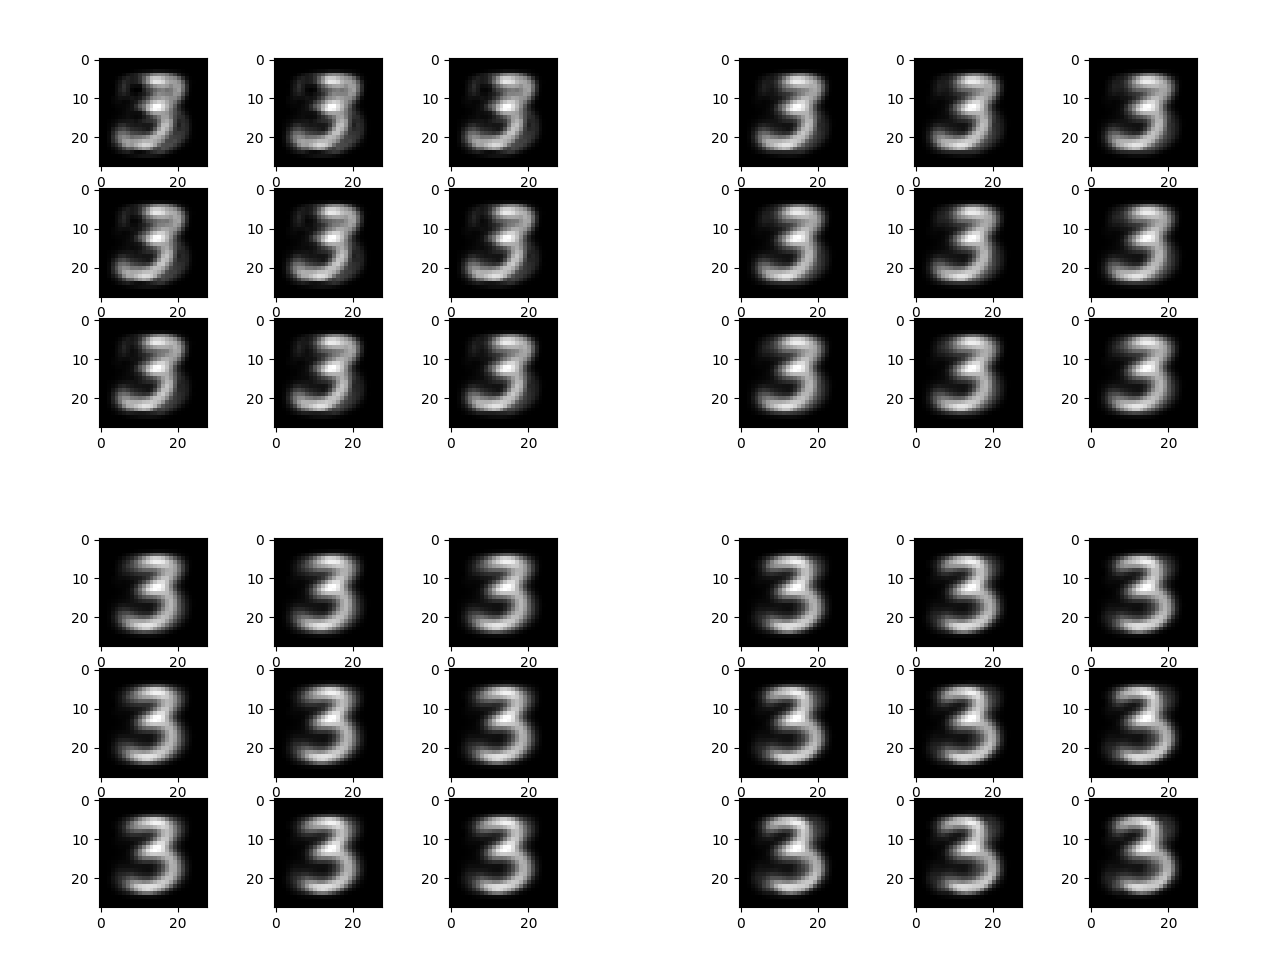
\includegraphics[scale=0.35]{main_mnist.png}
        \caption{MNIST Flows, from left to right.}
        \label{fig:mnistflows}
    \end{center}
\end{figure}\\
These images, read from left to right, top to bottom, are points from the greedy principal 
flow using the binary kernel. Although it does not represent 
all the variability of the 3s in the dataset, we can see that 
all the images obtained are "nice" representations of 3s, 
in that they cannot be confused with any other digit, and they seem to be relatively
neatly written. Within these "nice" 3s then we observe the source of the variability:
the "slant" of the digit. We can see that the digits start out 
leaning right with the upper left group of images,  and slowly rotates
to slant to the left, going through a phase of being perfectly centered, while the
tails of the images seem not to move at all. \\
This perhaps is an insight into the well-written 3s in the dataset and perhaps 
of neat handwritten digits in general: that the upper and middle part of the
digit differ mainly in orientation, while the tail remains mostly fixed.
Additionally, the fact that the 3s from the principal flow 
are neat representations of the digit, and the gradual change in
orientation of the digit along the curve suggests that our 
greedy principal flow has found a path that has some intuitive meaning.
This supports our use of the greedy principal flow to understand
our data better, and seek out some pattern of variation
that we might otherwise be oblivious too.
It also perhaps justifies our choice of a hypersphere for $\mathcal{M}^d$.

\iffalse
\subsection{Fashion MNIST}

Next we test our principal flow on objects, and rather on 2 pieces of fashion that
look quite alike: t-shirts and dresses.

\begin{figure}[ht]
    \begin{center}
        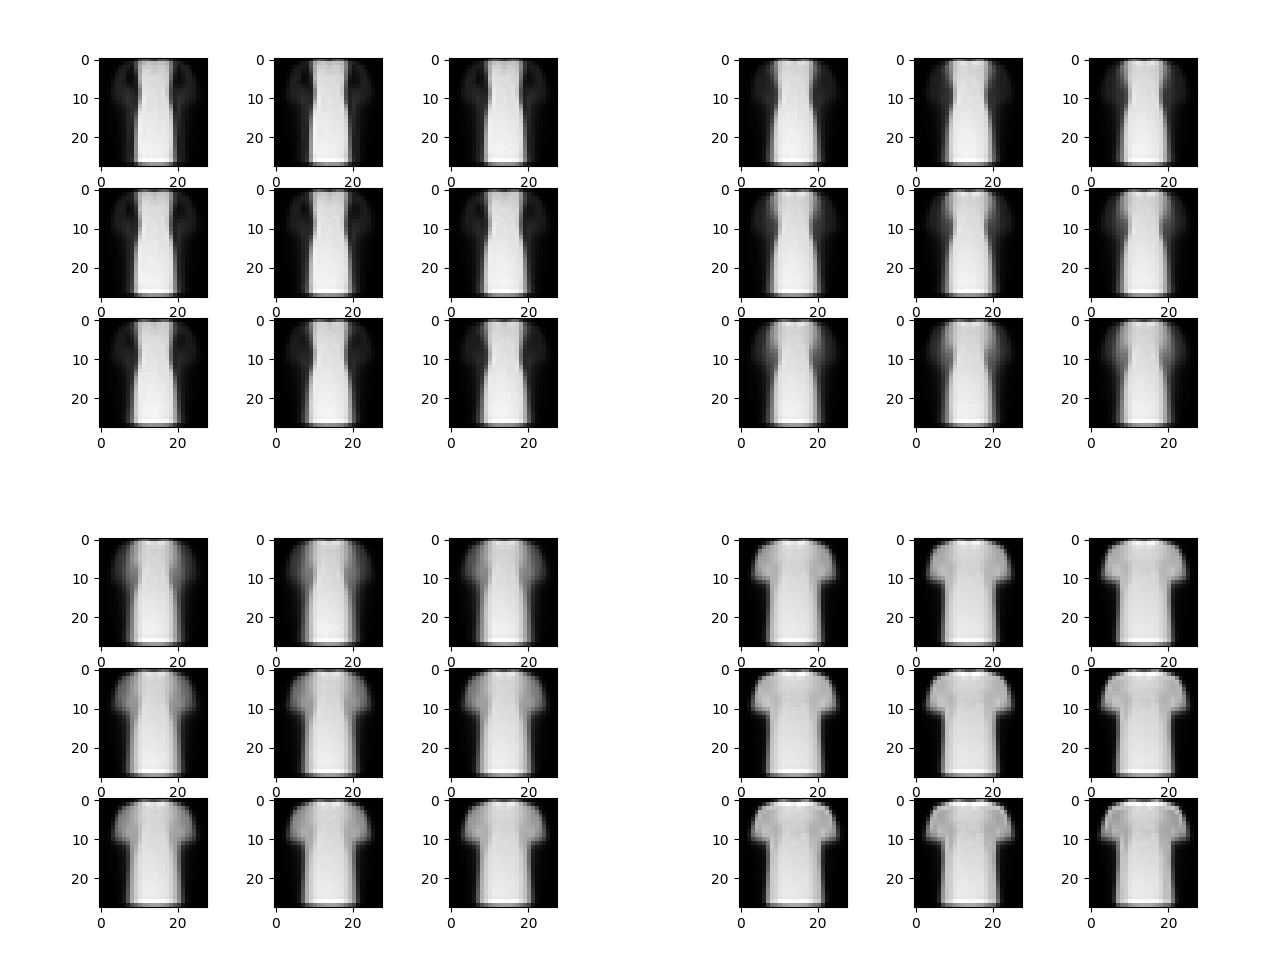
\includegraphics[scale=0.2]{main_fashion.png}
        \caption{Fasion MNIST Flows, from left to right.}
        \label{fig:fashionmnistflows}
    \end{center}
\end{figure}

Here we can watch as dresses morph into t-shirts. More than just an interesting graphic,
it shows that the principal flow is able to capture the variability of the data:
here the data varies very clearly in the outline of the images, and images on the
principal flow reflect this main source of variability.
\fi
\newpage
\subsection{Olivetti faces}

Next we test our algorithm on a facial dataset. The Olivetti face dataset is old,
and thus images are small, and only in black and white. This however is 
an advantage, as smaller images help the principal flow algorithm run faster,
allowing us to experiment with a variety of parameters.\\
\begin{figure}[ht]
    \begin{center}
        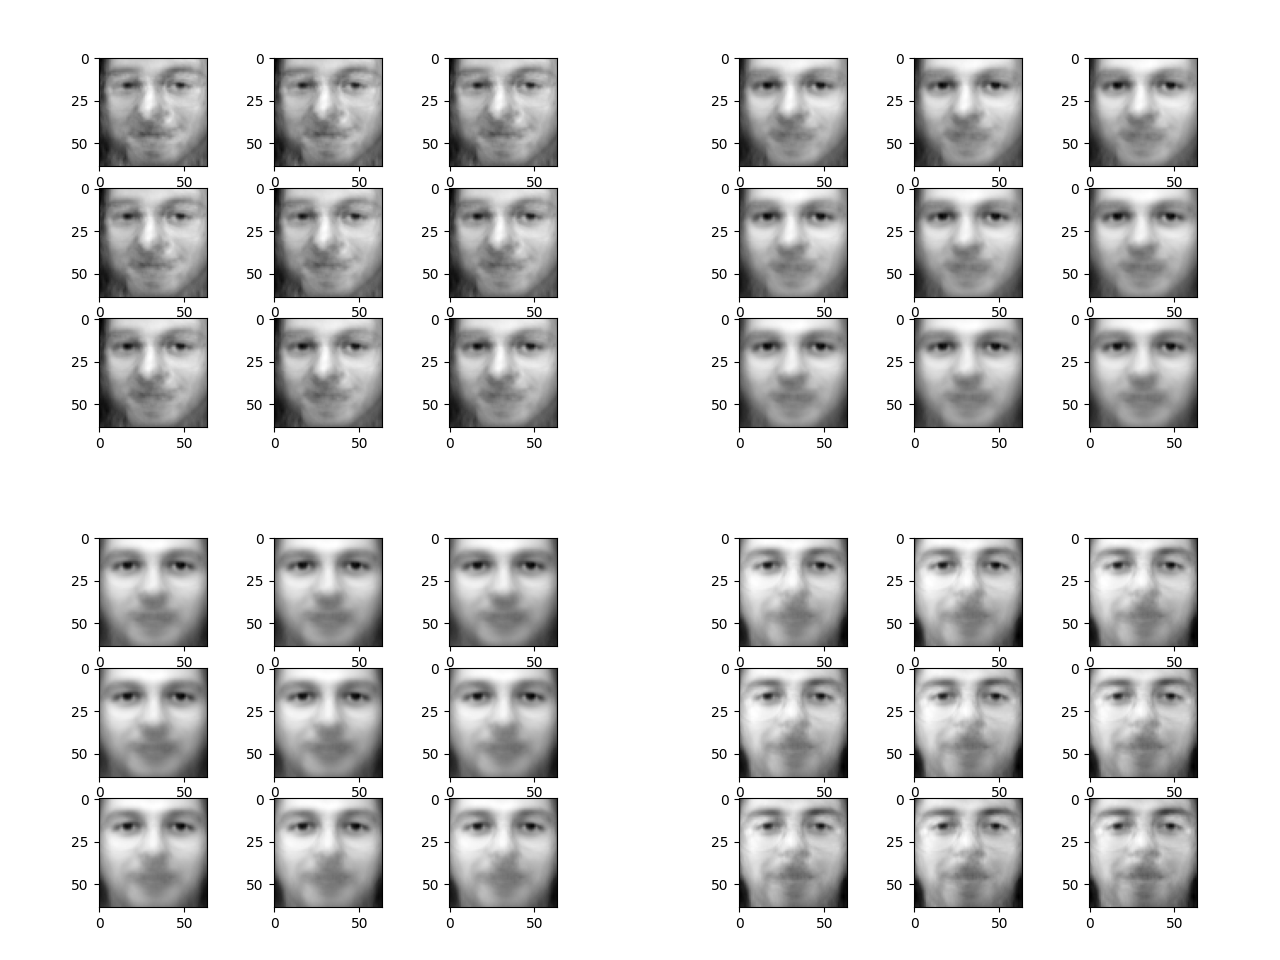
\includegraphics[scale=0.35]{main_olivetti_30_01.png}
        \caption{Flow for Olivetti face data, from left to right.}
        \label{fig:olivettiflows}
    \end{center}
\end{figure}\\
Although disturbing, we can see the results of our algorithm. 
We obtain mostly clear pictures of faces, with faces differing
in whether they wear glasses (first few images on upper left) or 
the angle of their face, or whether they have a beard (last two images, 
bottom right). Indeed
we observe that the difference between the men and woman in the data are not as stark
as the difference between bearded and non-bearded individuals. 
This again indicates the strength of our algorithm: it is able to suss out the 
main way in which these images vary.
Additionally, we can glean meaning from neighbouring images on the curve:
they are close to each other in a meaningful way. This can be seen from how the set 
of faces on the upper left are slightly tilted away from us, but gradually 
transition to facing us in the bottom left set of images.
The fact that the images on the principal flow
transition smoothly tell us that on the principal flow,
a face slightly tilted away is near a face directly facing
the camera which makes intuitive, real world sense.
This is an indication that our choice of $\mathcal{M}^d$ does yield fruit and
have some real world meaning, and that our principal flow seems to preserve some
real world interpretation and meaning as it transitions smoothly through the orientation
of faces in the data.

\iffalse
\subsection{Cartoon Faces}

\begin{figure}[ht]
    \begin{center}
        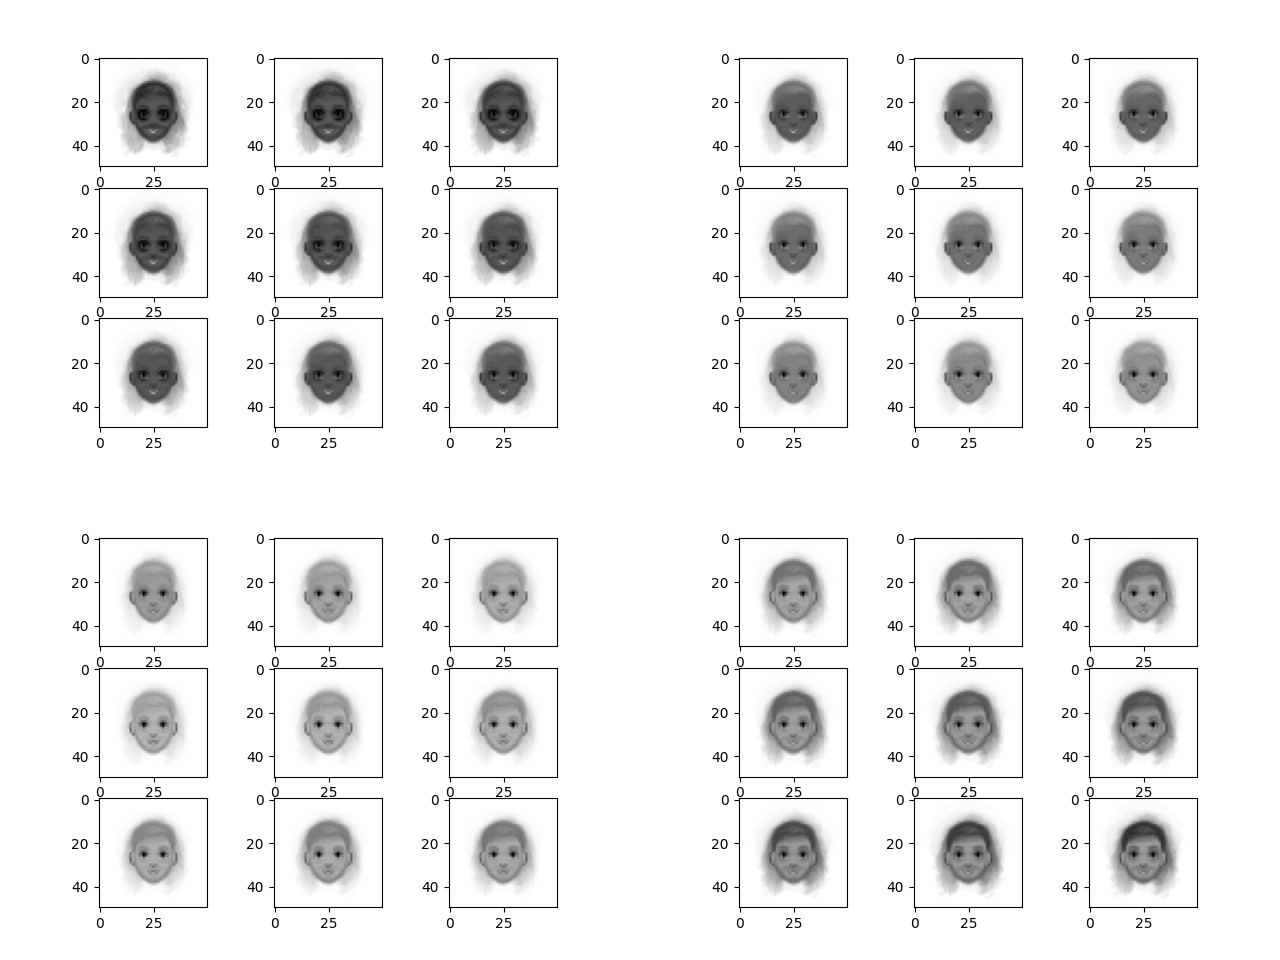
\includegraphics[scale=0.2]{main_cartoon_10_01.png}
        \caption{Cartoon face Flows, from left to right.}
        \label{fig:cartoonfaceflows1}
    \end{center}
\end{figure}

When run on a dataset of cartoon faces, the principal flow finds a series of 
faces that differ greatly in skin color and in hair color. Along the flow 
we can see that the faces start with a dark skin color and gradually 
transition to a lighter skin color, then get darker along with their hair color. 
Here we can see that faces vary mainly on skin tone and hair color, which makes intuitive sense, 
since other features like spectacles and a particular hair shape may not feature on many
data points.

\subsection{Faces in the Wild}
\begin{figure}[ht]
    \begin{center}
        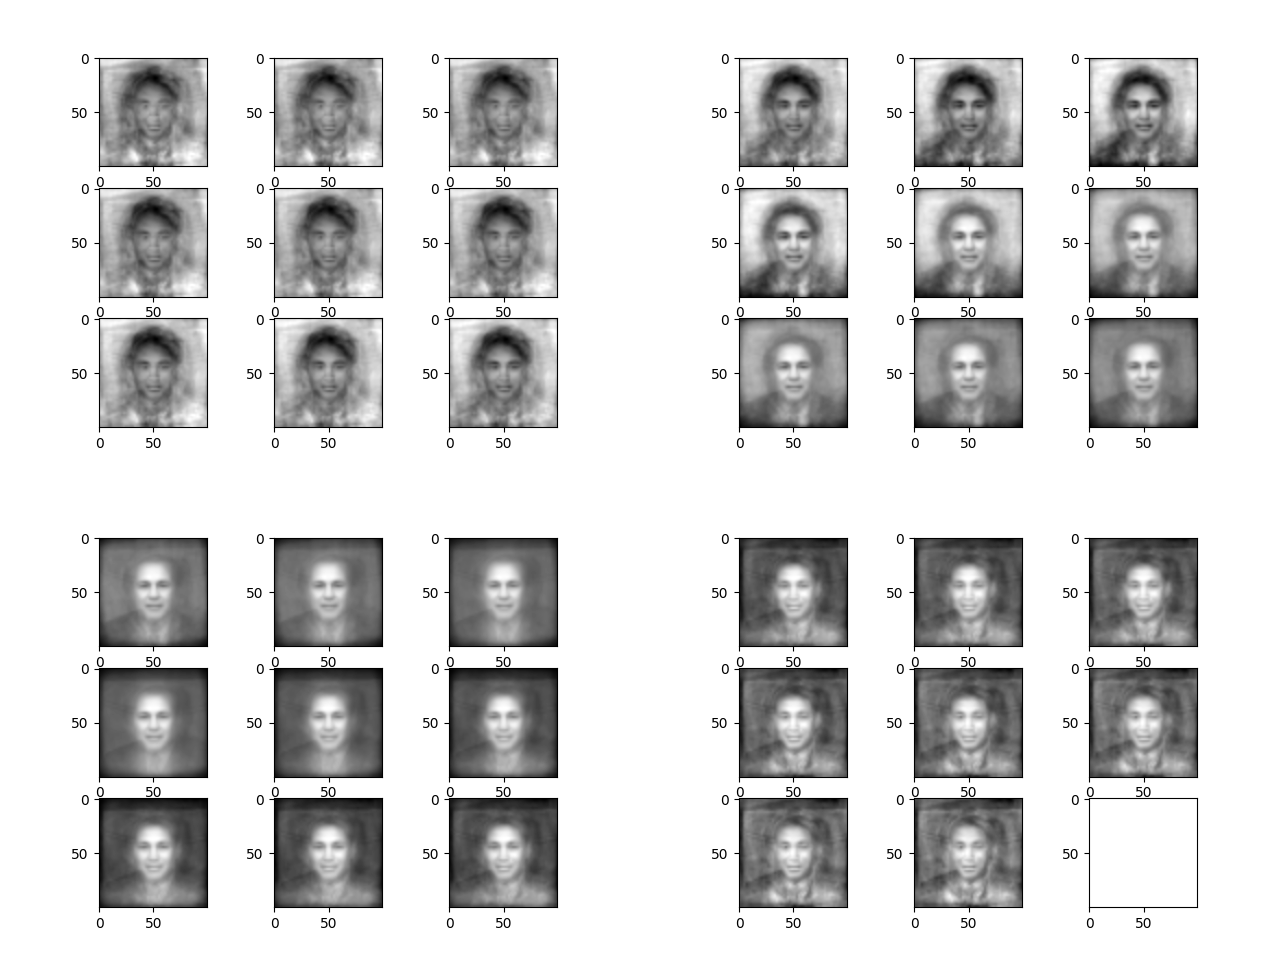
\includegraphics[scale=0.2]{main_lfw_10_05.png}
        \caption{Faces in the wild flow, from left to right.}
        \label{fig:cartoonfaceflows}
    \end{center}
\end{figure}

Here we test our principal flow algorithm on real faces with differing backgrounds, 
since these are photos found online. As with the cartoon faces, we can see that
these faces differ in skin tone but also in eyebrow color, eye shape and background. 
This makes intuitive sense, since skin tone will determine a large portion of the face,
and the background also takes up a large part of the images, and are likely to differ 
quite greatly.
\fi

\chapter*{Future Directions}

The topic of principal flows and manifold learning in general is a rich field 
with much potential, and there are many avenues of 
expanding the work done in this report. 
One potential direction is constructing the $k$-th order principal flows, where $k>1$. 
Another potential avenue of research is using different kinds of $\mathcal{M}^d$. 
In this report, we have restricted ourselves only to the hypersphere. Although this 
might be a "good enough" approximation, if we had intuition about the specific form 
of the manifold on which our multivariate data lies, and we determine that the 
hypersphere is unsuitable, then this current principal flow would not be able to 
accomodate this intuition. With a different manifold, we might be able to obtain 
a different principal flow that might give us more information about the 
variability of the data and describe it more appropriately than using the hypersphere. 
Additionally, we could also extend the greedy principal boundary to be a maximal margin
classifier. Although this has already been done in \cite{principalboundary}, 
it has yet to be done with a greedy approach, and would be the first
greedy maximal margin classifier for multivariate data lying on some 
Riemannian manifold.

\begin{thebibliography}{9}

\bibitem{mds}
Borg, I., and Groenen, P. J. F. (2005),
textit{Modern Multidimensional Scaling, Theory and Applications}, 
2 edn Springer.

\bibitem{pga}
Fletcher, P. T., Lu, C., Pizer, S. M., and Joshi, S. (2004), 
"Principal Geodesic Analysis for the Study of Nonlinear Statistics of Shape," 
\textit{IEEE Transactions on Medical Imaging}, 23, 995-1005.

\bibitem{isomap}
Tenenbaum, J. B., Silva, V. D., and Langford, J. C. (2000). "A Global
Geometric Framework for Nonlinear Dimensionality Reduction." 
\textit{Science}, 290: 2319-2323.

\bibitem{principalboundary}
Yao, Z., and Zhang, Z. (2019) "Principal Boundary on Riemannian Manifolds." 

\bibitem{principalflow}
Panaretos, V. M., Pham, T., and Yao, Z. (2014), 
"Principal Flows," \textit{Journal of the American
Statistical Association}, 109, 424-436.

\bibitem{lle}
Roweis, S. T., and Saul, L. K. (2003). “Think Globally, Fit Locally:
Supervised Learning of Low Dimensional Manifolds.” \textit{Journal of Machine
Learning Research}, 4: 119–155.

\bibitem{tanspaceimg}
Conrad Sanderson: Conceptual illustration of the tangent space at point P on a Riemannian manifold.
\\\texttt{\url{https://www.researchgate.net/figure/Conceptual-illustration-of-the-tangent-space-at
-point-P-on-a-Riemannian-manifold-M_fig2_262974373}}\\ Accessed: 03/03/2021

\bibitem{tanspaceimg2}
Alexwright: Tangent Space Illustration.\\
\texttt{}
\url{https://en.wikipedia.org/wiki/Tangent_space#/media/File:Image_Tangent-plane.svg}
Accessed: 03/03/2021
\end{thebibliography}


\end{document}